%!TEX root = ../thesis.tex
\chapter{Попередня обробка даних, побудова моделей та оцінка методів}
\label{chap:practice}

В даному розділі описано попередню обробку даних, які використовувалися в дослідженні, та описано параметри побудованих моделей. Також описано процес навчання та підбору гіперпараметрів моделей. Вказана перевірка моделей на тестових даних, за допомогою метрик: accuracy, precision, recall та f1-score.

\section{Попередня обробка даних}

Як вже зазначалося в даній роботі використовується три набори даних, а саме: Pima Indians Diabetes Database~\cite{ct30}, Human Activity Recognition with Smartphones~\cite{ct31} та Chest X-Ray Images (Pneumonia)~\cite{ct32}. Для кожного набору даних була застосована своя попередня обробка. Далі ми наведемо, які методи обробки були застосовані до кожного набору.

Почнемо розгляд з Pima Indians Diabetes Database (прочитати детальніше, про датасет можна у~\cite{ct30} або у розділі \ref{sec:data-description}). Першим кроком попередньої обробки була заміна нульових значень, які зустрічаються у деяких ознаках (Pregnancies, Glucose, BloodPressure, SkinThickness, Insulin, BMI, DiabetesPedigreeFunction, Age) на відсутні значення (nan). Це дозволяє уникнути впливу невірних даних на подальший аналіз. Далі, для кожної ознаки, у якої були відсутні значення, було обчислено медіанні значення для груп з позитивним та негативним результатом по діабету (Outcome). Відсутні значення заповнювалися відповідно до медіанної величини для відповідної групи. Після цього було проведено обробку змінної Insulin для видалення викидів. Викиди визначалися за допомогою методу Interquartile Range Technique~\cite{ct33}. Наступним кроком було виявлення та видалення викидів за допомогою методу Local Outlier Factor~\cite{ct34}. Цей метод використовує локальну щільність сусідів для визначення аномалій. Після розрахунку негативного фактору аномалії для кожного зразка, було визначено порогове значення, і видалено ті зразки, які мали значення нижче цього порогу. Після видалення аномалій дані були розділені на ознаки та мітки. Вибірки було поділено на тренувальний та тестовий набори даних у пропорції 80:20. Потім, для тренувального та тестового наборів даних було проведено стандартизацію ознак шляхом видалення середнього значення та масштабування до одиничної дисперсії. В результаті ми отримали оброблений датасет, який будемо використовувати для порівняння моделей для задачі бінарної класифікації табличних даних.

Наступну попередню обробку опишемо для набору даних Human Activity Recognition with Smartphones (прочитати детальніше, про датасет можна у~\cite{ct31} або у розділі \ref{sec:data-description}). Для цього набору даних було застосовано наступні методи попередньої обробки. По-перше, дані було розділено на тренувальну та тестову вибірки, кожна з яких містила відповідні дані для тренування та тестування моделей. Після завантаження датасетів для тренування та тестування, було застосовано LabelEncoder для кодування міток активностей (Activity) у числовий формат. Наступним кроком було розділення даних на ознаки та мітки для тренувальних і тестових вибірок. Далі було проведено випадкове перемішування тренувальних та тестових даних для уникнення впливу можливого порядку даних на результати навчання моделей. Для покращення роботи моделей було проведено стандартизацію ознак шляхом видалення середнього значення та масштабування до одиничної дисперсії. Цей процес дозволяє моделі краще адаптуватися до даних, які мають різний масштаб. В результаті попередньої обробки ми отримали стандартизовані та перемішані тренувальні та тестові набори даних, готові до подальшого використання у моделюванні. 

Нарешті, розглянемо попередню обробку даних для набору даних Chest X-Ray Images (Pneumonia) (прочитати детальніше про датасет можна у~\cite{ct32} або у розділі \ref{sec:data-description}). Для цього набору даних було застосовано наступні методи попередньої обробки. По-перше, дані були завантажені та організовані у вигляді класів, де кожне зображення має відповідну мітку (0 -- нормальний, 1 -- бактеріальна пневмонія, 2 -- вірусна пневмонія). Як зазначалося ми використали цей датасет для бінарної та багатокласової класифікації, для бінарної, відповідно, класи бактеріальна та вірусна пневмонії були об'єднані в один клас -- пневмонія, а для багатокласової використовувалися класи нормальний, бактеріальна пневмонія та вірусна пневмонія. Зображення були перетворені до розміру 224x224 пікселів і конвертовані в градації сірого для уніфікації формату. Для екстракції ознак було використано попередньо натреновану модель ResNet-50~\cite{ct35} без останнього повнозв'язного шару. Модель була завантажена зі збережених ваг (які ми самі натренували використовуючи цей же набір даних) та використана для отримання векторів ознак зображень. Далі, для обробки отриманих векторів ознак, було застосовано стандартизацію ознак шляхом видалення середнього значення та масштабування до одиничної дисперсії. Для зменшення розмірності та збереження 99$\%$ варіативності даних було застосовано метод Principal Component Analysis~\cite{ct36}. В результаті ми отримали оброблені вектори ознак, готові до подальшого використання у моделюванні.

\section{Детальний опис моделей та підбір гіперпараметрів моделей}

Як вже було зазначено в даній роботі ми сфокусувалися на тестуванні моделей MLP with gradient descent, MLP with single-point mutation та $(1+\lambda)$-EA with GP encodings. Принцип тренування MLP with gradient descent ми описали в розділі \ref{sec:training_process}, тому в цьому розділі ми опишемо детально процес навчання моделей MLP with single-point mutation та $(1+\lambda)$-EA with GP encodings.

MLP with single-point mutation використовує оптимізаційний алгоритм, який працює наступним чином: на кожній епосі випадковим чином обирається значення однієї ваги з усієї нейронної мережі та до нього додається значення випадкової величини, яка має нормальний розподіл з нульовим математичним сподіванням та певним значенням дисперсії, після цього розраховується функція втрат з оновленими вагами, якщо її значення стало менше, ніж було з початковими вагами на поточній епосі, то ваги зберігаються і процес переходить на наступну епоху, якщо функція втрат збільшилася, то повертаються ваги, які були до додавання значення випадкової величини і відбувається перехід на наступну епоху. Цей процес повторюється задану кількість епох.

Метод $(1+\lambda)$-EA with GP encodings описується наступним чином. Першим кроком ініціалізується індивід, в нашому випадку індивідом є дерево у якого в якості внутрішніх вузлів -- функції, які мають арність 2, а в якості листків -- features датасету або константи з набору: $1, 0, -1, e, \pi$. Для цього індивіду розраховується фітнес-функція. Після того, як була розрахована фітнес-функція для створеного індивіду, він мутує $\lambda$ разів, таким чином ми отримуємо $\lambda$ нових індивідів. Мутація в даному випадку відбувається наступним чином: випадково обирається один вузол з усього індивіду і його значення замінюється на якесь інше випадкове, валідне значення (у випадку внутрішніх вузлів -- значення замінюється на якусь іншу функцію, а у випадку листків на якусь іншу feature, або константу).  Після цього ми розраховуємо фітнес-функції для усіх новостворених індивідів і обираємо індивід, який має найменше значення фітнес-функцї. Цей індивід далі виступає в ролі батька на наступних ітераціях.

Тепер після того, як ми описали, як в нашому випадку працюють алгоритми, перейдемо до процесу підбору оптимальних гіперпараметрів. Процес вибору гіперпараметрів є важливим кроком в тренуванні моделей, оскільки від них значно залежить швидкість конвергенції та якість моделей. Тому в цій частині ми опишемо, процес за яким відбувається підбір гіперпараметрів для різних задач та моделей, а також які саме гіперпараметри виявилися найкращими і які ми використовуємо.

Почнемо розгляд з задач класифікації та моделі MLP with gradient descent. Для підбору гіперпараметрів для цієї моделі ми використовували бібліотеку optuna~\cite{ct22}, яка дозволяє проводити байєсівську оптимізацію~\cite{ct37}. Для цього ми задали простір гіперпараметрів по якому проводився пошук оптимальних з них за 1000 ітерацій. Найкращі гіперпараметри для кожної задачі можна подивитися у таблиці \ref{tab_hyperparameters_for_mlp_with_gd}.

\begin{table}[ht]
	\centering
	\begin{adjustbox}{max width=\textwidth}
		\begin{tabular}{|c|p{3cm}|p{3cm}|p{3cm}|p{3cm}|}
			\hline \multirow{2}{*}{Гіперпараметри} & \multicolumn{4}{c|}{Задачі} \\
			\cline{2-5} & Бінарна класифікація табличних даних & Бінарна класифікація картинок & Багатокласова класифікація табличних даних & Багатокласова класифікація картинок \\
			\hline hidden\_layer\_sizes & (10, 15, 10) & (15, 20, 15) & (10, 10) & (10, 10) \\
			\hline activation & tanh & tanh & logistic & tanh \\
			\hline solver & sgd & sgd & sgd & sgd \\
			\hline alpha & 0.0009 & 0.0054 & 0.0001 & 0.0001 \\
			\hline learning\_rate\_init & 0.004 & 0.002 & 0.008 & 0.001 \\
			\hline learning\_rate & adaptive & invscaling & adaptive & invscaling \\
			\hline batch\_size & 32 & 256 & 64 & 128 \\
			\hline tol & 0.00002 & 0.00033 & 0.00023 & 0.00003 \\
			\hline
		\end{tabular}
	\end{adjustbox}
	\caption{Найкращі гіперпараметри для моделі MLP with gradient descent}
	\label{tab_hyperparameters_for_mlp_with_gd}
\end{table}

Для моделі MLP with single-point mutation для пошуку оптимальних гіперпараметрів також було застосовану байєсівську оптимізацію~\cite{ct37} за 1000 ітерацій. В результаті ми отримали оптимальні гіперпараметри, які можна подивитися у таблиці \ref{tab_hyperparameters_for_mlp_with_sp_mut}.

\begin{table}[ht]
	\centering
	\begin{adjustbox}{max width=\textwidth}
		\begin{tabular}{|c|p{3cm}|p{3cm}|p{3cm}|p{3cm}|}
			\hline \multirow{2}{*}{Гіперпараметри} & \multicolumn{4}{c|}{Задачі} \\
			\cline{2-5} & Бінарна класифікація табличних даних & Бінарна класифікація картинок & Багатокласова класифікація табличних даних & Багатокласова класифікація картинок \\
			\hline hidden\_layer\_sizes & (10, 15, 20, 15, 10) & (15, 20, 15) & () & (10, 10) \\
			\hline scale\_for\_mutation & 0.5 & 0.1 & 0.1 & 0.1 \\
			\hline
		\end{tabular}
	\end{adjustbox}
	\caption{Найкращі гіперпараметри для моделі MLP with single-point mutation}
	\label{tab_hyperparameters_for_mlp_with_sp_mut}
\end{table}

Останньою моделлю для якої ми шукали оптимальні параметри є $(1+\lambda)$-EA with GP encoding. Процес пошуку такий же самий як і для вище наведених моделей. Відповідні результати наводяться у таблиці \ref{tab_hyperparameters_for_evol_alg}.

\begin{table}[ht]
	\centering
	\begin{adjustbox}{max width=\textwidth}
		\begin{tabular}{|c|p{3cm}|p{3cm}|p{3cm}|p{3cm}|}
			\hline \multirow{2}{*}{Гіперпараметри} & \multicolumn{4}{c|}{Задачі} \\
			\cline{2-5} & Бінарна класифікація табличних даних & Бінарна класифікація картинок & Багатокласова класифікація табличних даних & Багатокласова класифікація картинок \\
			\hline tree\_depth & 3 & 6 & 6 & 8 \\
			\hline $\lambda$ & 3 & 5 & 3 & 5 \\
			\hline
		\end{tabular}
	\end{adjustbox}
	\caption{Найкращі гіперпараметри для моделі $(1+\lambda)$-EA with GP encoding}
	\label{tab_hyperparameters_for_evol_alg}
\end{table}

Таким чином після того, як ми отримали оптимальні гіперпараметри для усіх моделей можна переходити до процесу тренування та аналізу результатів.

\section{Навчання моделей та порівняльний аналіз результатів}

Для тренування моделей ми використовуємо функції \ref{eq:binary_cross_entropy} та \ref{eq:cross_entropy} в якості функцій втрат для MLP та фітнес-функцій для $(1+\lambda)$-EA with GP encoding для бінарної та багатокласової класифікацій відповідно. Таким чином наші моделі вчаться мінімізувати ці функції, оскільки, як можна бачити, чим менше значення цих функцій тим більш правильний результат. Справді, підставивши в ці функції в якості $y_i$ -- 1 та в якості ймовірності $p_i$ також 1 (тобто це той випадок, коли справжня мітка для поточного прикладу -- 1 і модель на виході дає ймовірність того, що поточний приклад належить до класу 1 також 1), отримаємо: $1 \log(1) + (1 - 1) \log(1 - 1) = 0$, а якщо підставити в якості $y_i$ -- 0, а в якості ймовірності $p_i$ також 0 (тобто це той випадок, коли справжня мітка для поточного прикладу -- 0 і модель на виході дає ймовірність того, що поточний приклад належить до класу 1 також 0), отримаємо: $0 \log(0) + (1 - 0) \log(1 - 0) = 0$, що показує, що якщо модель правильно передбачила результат для прикладу, то значення функції втрат дорівнює 0. Для функції втрат для багатокласової класифікації подібна підстановка тільки з кількістю класів більше 2 також покаже, що функція втрат буде дорівнювати 0. Ще раз підсумовуючи, чим ближче функція втрат до 0, тим більш правильні передбачення робить модель, тобто під час навчання моделей стоїть задача саме мінімізувати функції втрат.

Для оцінки якості моделей ми використовували метрики зазначені в таблиці \ref{tab_metrics}. Опис які метрики в яких випадках краще використовувати можна прочитати в розділі \ref{sec:metrics}. Зазначимо, як видно з формул цих метрик чим ближче кожна з них до 1, тим більш якісніша модель. У випадку accuracy, якщо частина доданку в знаменнику, а саме $FP+FN$ буде дорівнювати 0, тобто наша модель не дасть жодного неправильного передбачення, то чисельник і знаменник будуть дорівнювати один одному, а отже значення accuracy буде 1, у випадку precision та recall, якщо частини доданків в знаменнику, а саме $FP$ та $FN$ будуть дорівнювати 0, тобто наша модель не дасть жодного неправильного результату, то чисельники та знаменники відповідних формул будуть рівні між собою, а отже і значення цих метрик буде дорівнювати 1 і остання метрика f1-score, підставивши в цю формулу $2 \times \frac{\text{Precision} \times \text{Recall}}{\text{Precision} + \text{Recall}}$ найкращі показники для precision та recall, а саме 1 та 1 отримаємо $2 \times \frac{1 \times 1}{1 + 1}$, що дорівнює 1.

Володіючи детальною інформацією про метрики та функції втрат перейдемо до тренування моделей. Почнемо розгляд з задачі бінарної класифікації табличних даних, як вже зазначалося в розділі \ref{sec:data-description} для цього ми використовували датасет Pima Indians Diabetes Database~\cite{ct30}. Оптимальні гіперпараметри для усіх трьох моделей можна знайти у попередньому розділі. Зазначимо, що MLP with gradient descent, MLP with single-point mutation та $(1+\lambda)$-EA with GP encodings тренувалися протягом 150, 6000 та 50 епох відповідно. Після тренування ми отримали результати для моделі MLP with gradient descent, які можна подивитися в таблиці \ref{mlp_gd_bc_td_results}, для моделі MLP with single-point mutation -- у таблиці \ref{mlp_spm_bc_td_results}, для моделі $(1+\lambda)$-EA with GP encodings -- у таблиці \ref{ea_bc_td_results}. Результуючі метрики на найкращій ітерації для усіх трьох моделей знаходяться в таблиці \ref{metrics_bc_td_results}. Графіки зміни функцій втрат для кожної моделі можна знайти на рисунку \ref{fig_losses_bc_td}

\begin{table}[ht]
	\centering
	\begin{adjustbox}{max width=\textwidth}
		\begin{tabular}{|c|c|c|c|}
			\hline 
			Номер епохи & Час тренування, секунди & Функція втрат для тренувальної вибірки & Функція втрат для тестувальної вибірки \\
			\hline 
			50 & 0.221 & 0.3327 & 0.3624 \\
			\hline 
			100 & 0.4406 & 0.2843 & 0.3302 \\
			\hline
			134 & 0.5883 & 0.2627 & 0.3236 \\
			\hline
			150 & 0.6578 & 0.2552 & 0.3244 \\
			\hline
		\end{tabular}
	\end{adjustbox}
	\caption{Результати моделі MLP with gradient descent для задачі бінарної класифікації табличних даних}
	\label{mlp_gd_bc_td_results}
\end{table}

\begin{table}[ht]
	\centering
	\begin{adjustbox}{max width=\textwidth}
		\begin{tabular}{|c|c|c|c|}
			\hline 
			Номер епохи & Час тренування, секунди & Функція втрат для тренувальної вибірки & Функція втрат для тестувальної вибірки \\
			\hline 
			1000 & 1.6075 & 0.6145 & 0.6068 \\
			\hline 
			2000 & 3.1348 & 0.4003 & 0.3845 \\
			\hline
			3000 & 4.6372 & 0.3476 & 0.37 \\
			\hline
			4000 & 6.1426 & 0.3096 & 0.3476 \\
			\hline
			5000 & 7.6502 & 0.2899 & 0.3331 \\
			\hline
			5377 & 8.2214 & 0.2805 & 0.3203 \\
			\hline
			6000 & 9.1574 & 0.2712 & 0.337 \\
			\hline
		\end{tabular}
	\end{adjustbox}
	\caption{Результати моделі MLP with single-point mutation для задачі бінарної класифікації табличних даних}
	\label{mlp_spm_bc_td_results}
\end{table}

\begin{table}[ht]
	\centering
	\begin{adjustbox}{max width=\textwidth}
		\begin{tabular}{|c|c|c|c|}
			\hline 
			Номер епохи & Час тренування, секунди & Функція втрат для тренувальної вибірки & Функція втрат для тестувальної вибірки \\
			\hline 
			10 & 0.1342 & 0.5605 & 0.5855 \\
			\hline 
			20 & 0.2827 & 0.476 & 0.4793 \\
			\hline
			30 & 0.4323 & 0.466 & 0.4867 \\
			\hline
			40 & 0.582 & 0.4493 & 0.4671 \\
			\hline
			44 & 0.6418 & 0.4056 & 0.4131 \\
			\hline
			50 & 0.7326 & 0.4056 & 0.4131 \\
			\hline
		\end{tabular}
	\end{adjustbox}
	\caption{Результати моделі $(1+\lambda)$-EA with GP encodings для задачі бінарної класифікації табличних даних}
	\label{ea_bc_td_results}
\end{table}

\begin{table}[ht]
	\centering
	\begin{adjustbox}{max width=\textwidth}
		\begin{tabular}{|c|c|c|c|}
			\hline 
			 & MLP with gradient descent & MLP with single-point mutation & $(1+\lambda)$-EA with GP encodings \\
			\hline 
			Accuracy & 0.8421 & 0.8618 & 0.8882 \\
			\hline 
			Precision & 0.7121 & 0.8 & 0.8148 \\
			\hline
			Recall & 0.9038 & 0.7843 & 0.8627 \\
			\hline
			F1-score & 0.7966 & 0.7921 & 0.8381 \\
			\hline
		\end{tabular}
	\end{adjustbox}
	\caption{Метрики на найкращій ітерації кожної моделі для задачі бінарної класифікації табличних даних}
	\label{metrics_bc_td_results}
\end{table}

\begin{figure}[ht]
	\centering
	\begin{subfigure}[b]{0.32\textwidth}    
		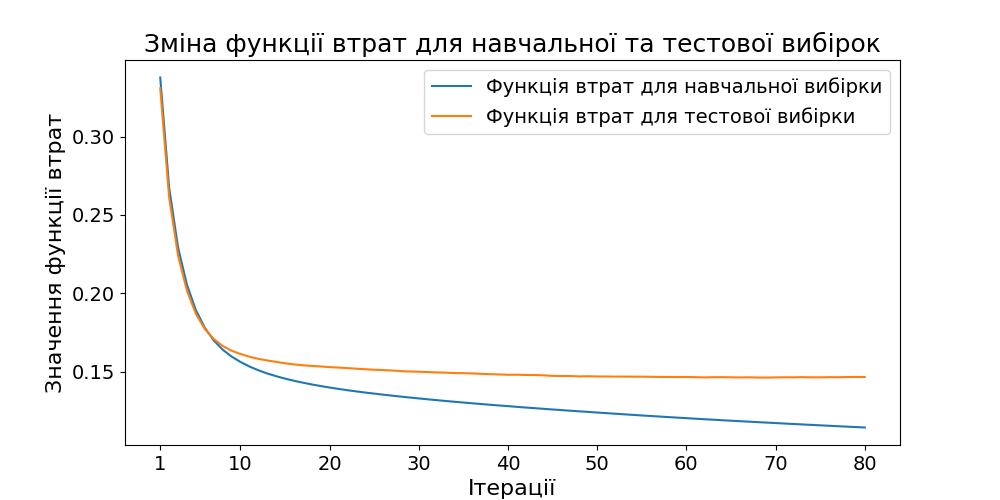
\includegraphics[width=\textwidth]{/home/loipoi/bachelor-diploma/pictures/binary_classification_tabular/mlp_with_gd_without_overfit.png}
		\caption{}
	\end{subfigure}
	\begin{subfigure}[b]{0.32\textwidth}
		\includegraphics[width=\textwidth]{/home/loipoi/bachelor-diploma/pictures/binary_classification_tabular/mlp_with_spm.png}
		\caption{}
	\end{subfigure}	
	\begin{subfigure}[b]{0.32\textwidth}
		\includegraphics[width=\textwidth]{/home/loipoi/bachelor-diploma/pictures/binary_classification_tabular/ea.png}
		\caption{}
	\end{subfigure}
	
	\caption{Графіки залежності функцій втрат від кількості ітерацій для методів: (a) MLP with gradient descent, (б) MLP with single-point mutation, (в) $(1+\lambda)$-EA with GP encodings, для задачі бінарної класифікації табличних даних}
	\label{fig_losses_bc_td}
\end{figure}

Як видно з цих даних, усі три моделі можуть досягти приблизно однакових метрик, найкращі результати моделі MLP with gradient descent, MLP with single-point mutation та $(1+\lambda)$-EA with GP encodings мали після 134, 5377 та 44 епох відповідно, але якщо говорити в термінах часу, то на цих даних найкраще себе показали моделі MLP with gradient descent та $(1+\lambda)$-EA with GP encodings, час роботи, яких склав 0.5883 та 0.6418 секунд відповідно, в той час, як алгоритму MLP with single-point mutation знадобилось значно більше часу, щоб зійтися до таких же метрик -- 8.2214 секунд.

Тепер перейдемо до задачі бінарної класифікації картинок. Як ми вже згадували у розділі \ref{sec:data-description} для цього ми використовували датасет Chest X-Ray Images (Pneumonia)~\cite{ct32}. Оптимальні гіперпараметри для усіх трьох моделей можна знайти у попередньому розділі. Зазначимо, що моделі тренувалися протягом 80, 6000 та 350 епох відповідно. Після тренування ми отримали результати для моделі MLP with gradient descent, які можна подивитися в таблиці \ref{mlp_gd_bc_id_results}, для моделі MLP with single-point mutation -- у таблиці \ref{mlp_spm_bc_id_results}, для моделі $(1+\lambda)$-EA with GP encodings -- у таблиці \ref{ea_bc_id_results}. Результуючі метрики на найкращій ітерації для усіх трьох моделей знаходяться в таблиці \ref{metrics_bc_id_results}. Графіки зміни функцій втрат для кожної моделі можна знайти на рисунку \ref{fig_losses_bc_id}.

\begin{table}[ht]
	\centering
	\begin{adjustbox}{max width=\textwidth}
		\begin{tabular}{|c|c|c|c|}
			\hline 
			Номер епохи & Час тренування, секунди & Функція втрат для тренувальної вибірки & Функція втрат для тестувальної вибірки \\
			\hline 
			20 & 0.4934 & 0.1398 & 0.1529 \\
			\hline 
			40 & 0.9766 & 0.128 & 0.148 \\
			\hline
			60 & 1.495 & 0.1203 & 0.1466 \\
			\hline
			69 & 1.7166 & 0.1175 & 0.1462 \\
			\hline
			80 & 1.972 & 0.1143 & 0.1465 \\
			\hline
		\end{tabular}
	\end{adjustbox}
	\caption{Результати моделі MLP with gradient descent для задачі бінарної класифікації картинок}
	\label{mlp_gd_bc_id_results}
\end{table}

\begin{table}[ht]
	\centering
	\begin{adjustbox}{max width=\textwidth}
		\begin{tabular}{|c|c|c|c|}
			\hline 
			Номер епохи & Час тренування, секунди & Функція втрат для тренувальної вибірки & Функція втрат для тестувальної вибірки \\
			\hline 
			1000 & 7.9608 & 0.5482 & 0.5476 \\
			\hline 
			2000 & 16.1285 & 0.4668 & 0.4662 \\
			\hline
			3000 & 24.144 & 0.3523 & 0.3514 \\
			\hline
			4000 & 32.0257 & 0.2365 & 0.2388 \\
			\hline
			5000 & 39.8537 & 0.1721 & 0.181 \\
			\hline
			5855 & 46.5702 & 0.1506 & 0.1696 \\
			\hline
			6000 & 47.7299 & 0.148 & 0.1703 \\
			\hline
		\end{tabular}
	\end{adjustbox}
	\caption{Результати моделі MLP with single-point mutation для задачі бінарної класифікації картинок}
	\label{mlp_spm_bc_id_results}
\end{table}

\begin{table}[ht]
	\centering
	\begin{adjustbox}{max width=\textwidth}
		\begin{tabular}{|c|c|c|c|}
			\hline 
			Номер епохи & Час тренування, секунди & Функція втрат для тренувальної вибірки & Функція втрат для тестувальної вибірки \\
			\hline 
			50 & 44.4377 & 0.5538 & 0.6334 \\
			\hline 
			100 & 88.4321 & 0.4843 & 0.5863 \\
			\hline
			150 & 137.0132 & 0.4676 & 0.5756 \\
			\hline
			200 & 222.5579 & 0.462 & 0.5659 \\
			\hline
			250 & 269.5155 & 0.4544 & 0.549 \\
			\hline
			300 & 312.1965 & 0.4473 & 0.5455 \\
			\hline
			314 & 324.0475 & 0.373 & 0.5282 \\
			\hline
			350 & 355.8637 & 0.3133 & 0.5942 \\
			\hline
		\end{tabular}
	\end{adjustbox}
	\caption{Результати моделі $(1+\lambda)$-EA with GP encodings для задачі бінарної класифікації картинок}
	\label{ea_bc_id_results}
\end{table}

\begin{table}[ht]
	\centering
	\begin{adjustbox}{max width=\textwidth}
		\begin{tabular}{|c|c|c|c|}
			\hline 
			& MLP with gradient descent & MLP with single-point mutation & $(1+\lambda)$-EA with GP encodings \\
			\hline 
			Accuracy & 0.9582 & 0.9539 & 0.8686 \\
			\hline 
			Precision & 0.9681 & 0.9665 & 0.8649 \\
			\hline
			Recall & 0.9754 & 0.9709 & 0.9359 \\
			\hline
			F1-score & 0.9716 & 0.9687 & 0.899 \\
			\hline
		\end{tabular}
	\end{adjustbox}
	\caption{Метрики на найкращій ітерації кожної моделі для задачі бінарної класифікації картинок}
	\label{metrics_bc_id_results}
\end{table}

\begin{figure}[ht]
	\centering
	\begin{subfigure}[b]{0.32\textwidth}    
		\includegraphics[width=\textwidth]{/home/loipoi/bachelor-diploma/pictures/binary_classification_image/mlp_with_gd.png}
		\caption{}
	\end{subfigure}	
	\begin{subfigure}[b]{0.32\textwidth}
		\includegraphics[width=\textwidth]{/home/loipoi/bachelor-diploma/pictures/binary_classification_image/mlp_with_spm.png}
		\caption{}
	\end{subfigure}	
	\begin{subfigure}[b]{0.32\textwidth}
		\includegraphics[width=\textwidth]{/home/loipoi/bachelor-diploma/pictures/binary_classification_image/ea.png}
		\caption{}
	\end{subfigure}
	
	\caption{Графіки залежності функцій втрат від кількості ітерацій для методів: (a) MLP with gradient descent, (б) MLP with single-point mutation, (в) $(1+\lambda)$-EA with GP encodings, для задачі бінарної класифікації картинок}
	\label{fig_losses_bc_id}
\end{figure}

З цих результатів можна бачити, що усі три моделі досягають приблизно однакових метрик. Найкращі результати моделі MLP with gradient descent, MLP with single-point mutation та $(1+\lambda)$-EA with GP encodings мали після 4, 4067 та 314 епох відповідно, але якщо проаналізувати часову складову результатів, то видно, що модель MLP with gradient descent має доволі гарні результати, а саме найкращий показник функції втрат на тестовій вибірці до якого модель зійшлась за 0.2421 секунди, в той час, як моделі MLP with single-point mutation та $(1+\lambda)$-EA with GP encodings зійшлись до приблизно таких же показників за значно більший час, а саме 34.1213 та 324.0475 секунд відповідно. Варто зазначити, що модель MLP with gradient descent отримала такі гарні показники за доволі малу кількість ітерацій -- 4, це говорить про те, що початкова ініціалізація, яку ми використовуємо добре підходить для цієї задачі, або що функція втрат гладка, що також є великим плюсом для алгоритмів з оптимізаційним алгоритмом в основі якого градієнтний спуск (детальніше про це буде далі в цьому розділі).

Тепер розглянемо задачу багатокласової класифікації табличних даних. Як вже згадувалося у розділі \ref{sec:data-description} для цього ми використовували датасет Human Activity Recognition with Smartphones~\cite{ct31}. Оптимальні гіперпараметри для усіх трьох моделей можна знайти у попередньому розділі. Зазначимо, що моделі тренувалися протягом 100, 40000 та 15000 епох відповідно. Після тренування ми отримали результати для моделі MLP with gradient descent, які можна знайти у таблиці \ref{mlp_gd_mc_td_results}, для моделі MLP with single-point mutation -- у таблиці \ref{mlp_spm_mc_td_results}, для моделі $(1+\lambda)$-EA with GP encodings -- у таблиці \ref{ea_mc_td_results}. Результуючі метрики на найкращій ітерації для усіх трьох моделей знаходяться в таблиці \ref{metrics_mc_td_results}. Графіки зміни функцій втрат для кожної моделі можна знайти на рисунку \ref{fig_losses_mc_td}.

\begin{table}[ht]
	\centering
	\begin{adjustbox}{max width=\textwidth}
		\begin{tabular}{|c|c|c|c|}
			\hline 
			Номер епохи & Час тренування, секунди & Функція втрат для тренувальної вибірки & Функція втрат для тестувальної вибірки \\
			\hline 
			20 & 1.1138 & 1.0118 & 1.0082\\
			\hline 
			40 & 2.1845 & 0.4628 & 0.5151 \\
			\hline
			60 & 3.2554 & 0.0901 & 0.1978 \\
			\hline
			80 & 4.3575 & 0.0473 & 0.1823 \\
			\hline
			100 & 5.6244 & 0.0339 & 0.1749 \\
			\hline
		\end{tabular}
	\end{adjustbox}
	\caption{Результати моделі MLP with gradient descent для задачі багатокласової класифікації табличних даних}
	\label{mlp_gd_mc_td_results}
\end{table}

\begin{table}[ht]
	\centering
	\begin{adjustbox}{max width=\textwidth}
		\begin{tabular}{|c|c|c|c|}
			\hline 
			Номер епохи & Час тренування, секунди & Функція втрат для тренувальної вибірки & Функція втрат для тестувальної вибірки \\
			\hline 
			10000 & 100.6342 & 0.1509 & 0.2156 \\
			\hline 
			20000 & 197.7918 & 0.0743 & 0.1443 \\
			\hline
			30000 & 297.6863 & 0.0507 & 0.1371 \\
			\hline
			30355 & 301.4574 & 0.0502 & 0.1331 \\
			\hline
			40000 & 392.262 & 0.0427 & 0.1388 \\
			\hline
		\end{tabular}
	\end{adjustbox}
	\caption{Результати моделі MLP with single-point mutation для задачі багатокласової класифікації табличних даних}
	\label{mlp_spm_mc_td_results}
\end{table}

\begin{table}[ht]
	\centering
	\begin{adjustbox}{max width=\textwidth}
		\begin{tabular}{|c|c|c|c|}
			\hline 
			Номер епохи & Час тренування, секунди & Функція втрат для тренувальної вибірки & Функція втрат для тестувальної вибірки \\
			\hline 
			5000 & 36851.8799 & 0.1944 & 0.4746 \\
			\hline 
			10000 & 74160.3937 & 0.109 & 0.4322 \\
			\hline
			13151 & 98058.2898, & 0.0906 & 0.3413 \\
			\hline
			15000 & 112014.1368 & 0.0801 & 0.405 \\
			\hline
		\end{tabular}
	\end{adjustbox}
	\caption{Результати моделі $(1+\lambda)$-EA with GP encodings для задачі багатокласової класифікації табличних даних}
	\label{ea_mc_td_results}
\end{table}

\begin{table}[ht]
	\centering
	\begin{adjustbox}{max width=\textwidth}
		\begin{tabular}{|c|c|c|c|}
			\hline 
			& MLP with gradient descent & MLP with single-point mutation & $(1+\lambda)$-EA with GP encodings \\
			\hline 
			Accuracy & 0.9389 & 0.9532 & 0.8992 \\
			\hline 
			Precision & 0.9409 & 0.954 & 0.9024 \\
			\hline
			Recall & 0.9389 & 0.9532 & 0.8992 \\
			\hline
			F1-score & 0.9386 & 0.953 & 0.8994 \\
			\hline
		\end{tabular}
	\end{adjustbox}
	\caption{Метрики на найкращій ітерації кожної моделі для задачі багатокласової класифікації табличних даних}
	\label{metrics_mc_td_results}
\end{table}

\begin{figure}[ht]
	\centering
	\begin{subfigure}[b]{0.32\textwidth}    
		\includegraphics[width=\textwidth]{/home/loipoi/bachelor-diploma/pictures/multiclass_classification_tabular/mlp_with_gd.png}
		\caption{}
	\end{subfigure}	
	\begin{subfigure}[b]{0.32\textwidth}
		\includegraphics[width=\textwidth]{/home/loipoi/bachelor-diploma/pictures/multiclass_classification_tabular/mlp_with_spm.png}
		\caption{}
	\end{subfigure}	
	\begin{subfigure}[b]{0.32\textwidth}
		\includegraphics[width=\textwidth]{/home/loipoi/bachelor-diploma/pictures/multiclass_classification_tabular/ea.png}
		\caption{}
	\end{subfigure}
	
	\caption{Графіки залежності функцій втрат від кількості ітерацій для методів: (a) MLP with gradient descent, (б) MLP with single-point mutation, (в) $(1+\lambda)$-EA with GP encodings, для задачі багатокласової класифікації табличних даних}
	\label{fig_losses_mc_td}
\end{figure}

З цих результатів можна бачити, що моделі MLP with gradient descent та MLP with single-point mutation показали трохи кращі результати за $(1+\lambda)$-EA with GP encodings, але метод $(1+\lambda)$-EA with GP encodings виділився легкістю контролювання, оскільки для покращення його метрик нам потрібно просто збільшити експресивність кодувань, а саме збільшити значення гіперпараметрів tree\_depth, або $\lambda$, в той час, щоб покращити значення метрик методів MLP with gradient descent та MLP with single-point mutation нам потрібно робити оптимізацію гіперпараметрів, у першому випадку нам потрібно буде підбирати параметри, які наведені у таблиці \ref{tab_hyperparameters_for_mlp_with_gd}, а для другого випадку потрібно буде підбирати значення гіперпараметрів з таблиці \ref{tab_hyperparameters_for_mlp_with_sp_mut} (більш детальніше про це буде далі в цьому розділі). Найкращі результати моделі MLP with gradient descent, MLP with single-point mutation та $(1+\lambda)$-EA with GP encodings мали після 100, 30355 та 13151 епох відповідно, але якщо проаналізувати часову складову результатів, то видно, що модель MLP with gradient descent має значно кращі результати, ніж два інші методи, а саме найкращий показник функції втрат на тестовій вибірці до якого модель зійшлась за 5.6244 секунд, в той час, як моделі MLP with single-point mutation та $(1+\lambda)$-EA with GP encodings зійшлись до приблизно таких же показників за значно більший час, а саме 301.4574 та 98058.2898 секунд відповідно. Тобто бачимо, що час, який знадобився моделі $(1+\lambda)$-EA with GP encodings значно більший за час двох інших моделей.

Перейдемо до розгляду останньої задачі для якої ми робили порівняння моделей, а саме багатокласової класифікації картинок. Як ми вже згадували у розділі \ref{sec:data-description} для цього ми використовували датасет Chest X-Ray Images (Pneumonia)~\cite{ct32}. Оптимальні гіперпараметри для усіх трьох моделей можна знайти у попередньому розділі. Зазначимо, що моделі тренувалися протягом 4, 4000 та 3000 епох відповідно. Після тренування ми отримали результати для моделі MLP with gradient descent, які можна знайти у таблиці \ref{mlp_gd_mc_id_results}, для моделі MLP with single-point mutation -- у таблиці \ref{mlp_spm_mc_id_results}, для моделі $(1+\lambda)$-EA with GP encodings -- у таблиці \ref{ea_mc_id_results}. Результуючі метрики на найкращій ітерації для усіх трьох моделей знаходяться в таблиці \ref{metrics_mc_id_results}. Графіки зміни функцій втрат для кожної моделі можна знайти на рисунку \ref{fig_losses_mc_id}.

\begin{table}[ht]
	\centering
	\begin{adjustbox}{max width=\textwidth}
		\begin{tabular}{|c|c|c|c|}
			\hline 
			Номер епохи & Час тренування, секунди & Функція втрат для тренувальної вибірки & Функція втрат для тестувальної вибірки \\
			\hline 
			1 & 0.0743 & 0.6597 & 0.7961 \\
			\hline 
			2 & 0.1188 & 0.5825 & 0.7284 \\
			\hline
			3 & 0.1576 & 0.5474 & 0.7117 \\
			\hline
			4 & 0.1965 & 0.5275 & 0.7099 \\
			\hline
		\end{tabular}
	\end{adjustbox}
	\caption{Результати моделі MLP with gradient descent для задачі багатокласової класифікації картинок}
	\label{mlp_gd_mc_id_results}
\end{table}

\begin{table}[ht]
	\centering
	\begin{adjustbox}{max width=\textwidth}
		\begin{tabular}{|c|c|c|c|}
			\hline 
			Номер епохи & Час тренування, секунди & Функція втрат для тренувальної вибірки & Функція втрат для тестувальної вибірки \\
			\hline 
			1000 & 5.942 & 0.9455 & 1.0223 \\
			\hline 
			2000 & 11.8621 & 0.7553 & 0.868 \\
			\hline
			3000 & 17.8618 & 0.6136 & 0.8391 \\
			\hline
			3198 & 19.0337 & 0.5913 & 0.8258 \\
			\hline
			4000 & 23.8062 & 0.5163 & 0.898 \\
			\hline
		\end{tabular}
	\end{adjustbox}
	\caption{Результати моделі MLP with single-point mutation для задачі багатокласової класифікації картинок}
	\label{mlp_spm_mc_id_results}
\end{table}

\begin{table}[ht]
	\centering
	\begin{adjustbox}{max width=\textwidth}
		\begin{tabular}{|c|c|c|c|}
			\hline 
			Номер епохи & Час тренування, секунди & Функція втрат для тренувальної вибірки & Функція втрат для тестувальної вибірки \\
			\hline 
			1000 & 18508.0342 & 0.7506 & 0.8955 \\
			\hline 
			2000 & 36454.2143 & 0.6505 & 0.8406 \\
			\hline
			2382 & 43179.4566 & 0.623 & 0.823 \\
			\hline
			3000 & 53760.2125 & 0.5791 & 0.8661 \\
			\hline
		\end{tabular}
	\end{adjustbox}
	\caption{Результати моделі $(1+\lambda)$-EA with GP encodings для задачі багатокласової класифікації картинок}
	\label{ea_mc_id_results}
\end{table}

\begin{table}[ht]
	\centering
	\begin{adjustbox}{max width=\textwidth}
		\begin{tabular}{|c|c|c|c|}
			\hline 
			& MLP with gradient descent & MLP with single-point mutation & $(1+\lambda)$-EA with GP encodings \\
			\hline 
			Accuracy & 0.742 & 0.7356 & 0.6955 \\
			\hline 
			Precision & 0.7705 & 0.7677 & 0.7195 \\
			\hline
			Recall & 0.742 & 0.7356 & 0.6955 \\
			\hline
			F1-score & 0.7356 & 0.7288 & 0.6903 \\
			\hline
		\end{tabular}
	\end{adjustbox}
	\caption{Метрики на найкращій ітерації кожної моделі для задачі багатокласової класифікації картинок}
	\label{metrics_mc_id_results}
\end{table}

\begin{figure}[ht]
	\centering
	\begin{subfigure}[b]{0.32\textwidth}    
		\includegraphics[width=\textwidth]{/home/loipoi/bachelor-diploma/pictures/multiclass_classification_image/mlp_with_gd.png}
		\caption{}
	\end{subfigure}	
	\begin{subfigure}[b]{0.32\textwidth}
		\includegraphics[width=\textwidth]{/home/loipoi/bachelor-diploma/pictures/multiclass_classification_image/mlp_with_spm.png}
		\caption{}
	\end{subfigure}	
	\begin{subfigure}[b]{0.32\textwidth}
		\includegraphics[width=\textwidth]{/home/loipoi/bachelor-diploma/pictures/multiclass_classification_image/ea.png}
		\caption{}
	\end{subfigure}
	
	\caption{Графіки залежності функцій втрат від кількості ітерацій для методів: (a) MLP with gradient descent, (б) MLP with single-point mutation, (в) $(1+\lambda)$-EA with GP encodings, для задачі багатокласової класифікації картинок}
	\label{fig_losses_mc_id}
\end{figure}

З цих результатів можна бачити, що усі три моделі досягають приблизно однакових метрик. Найкращі результати моделі MLP with gradient descent, MLP with single-point mutation та $(1+\lambda)$-EA with GP encodings мали після 4, 3198 та 2382 епох відповідно. Проаналізувавши часову складову результатів видно, що модель MLP with gradient descent має доволі гарні результати, а саме найкращий показник функції втрат на тестовій вибірці до якого модель зійшлась за 0.1965 секунд, в той час, як моделі MLP with single-point mutation та $(1+\lambda)$-EA with GP encodings зійшлись до приблизно таких же показників за значно більший час, а саме 19.0337 та 43179.4566 секунд відповідно.

Провівши експерименти для чотирьох різних задач можна зробити висновок, що усі три методи можуть досягти однаково високих показників, або порівнюваних, але в кожного з методів є свої сильні та слабкі сторони. 

Модель MLP with gradient descent має швидкий час збіжності до точки оптимуму в порівнянні з іншими двома методами, але при цьому таку модель важко контролювати. Оскільки, якщо модель демонструє погані метрики, то ми не можемо точно сказати, як це покращити, чи збільшувати, наприклад, параметр learning\_rate, чи ні, оскільки через його збільшення модель може перескочити оптимальну точку, а через зменшення, навпаки дуже довго збігатися до неї, тому для того, щоб отримати гарні результати, потрібно проводити оптимізацію гіперпараметрів. Але в той же час, як ми бачили на прикладі класифікації картинок, якщо функція втрат доволі гладка і якщо початкова ініціалізація ваг достатньо вдала, то метод на основі градієнтного спуску доволі швидко збігається до точки оптимуму, це відбувається тому, що в цьому оптимізаційному методі, оптимізація параметрів моделі (а саме ваг та bias) відбувається в усіх напрямках, тобто за одну ітерацію кожен з параметрів зміщується в оптимальну сторону, навідмінну від методу MLP with single-point mutation, під час якого за одну ітерацію змінються значення тільки одних ваг, через це модель просто спускається до точки оптимуму одразу по усім осям. Таким чином, можна зробити висновок, що якщо для поточної задачі важлива швидкість навчання моделі, то MLP with gradient descent є гарним вибором, однак, якщо нам важливо мати контроль над моделлю, то краще обрати іншу модель.

Як видно з експериментів модель MLP with single-point mutation більш повільно збігається до точки оптимуму, ніж MLP with gradient descent, але в той же час не надто повільно. Але вона має перевагу в термінах контролювання, ця модель має значно менше гіперпараметрів для оптимізації, всього два: hidden\_layer\_sizes та scale\_for\_mutation. Хоча все одно важко сказати, як саме потрібно змінювати значення цих гіперпараметрів, якщо модель демонструє незадовільний результат, але за рахунок того, що гіперпараметрів значно менше, ніж у моделі MLP with gradient descent, зменшується простір пошуку гіперпараметрів, таким чином ми можемо за n кількість ітерацій пройти більше в глибину і підібрати більш кращі значення цих параметрів, ніж ми могли б це зробити з такою ж кількістю ітерацій, але для моделі MLP with gradient descent. Але як вже було зазначено, за одну ітерацію модель потенційно змінює тільки одне значення ваг, при чому це значення може виявитися гіршим, ніж те значення, яке було до цього, через що нове значення не прийметься, тобто за одну ітерацію значення взагалі в результаті може не змінитися, саме через це ця модель може значно довше збігається до точки оптимуму.

Останньою розглянемо модель $(1+\lambda)$-EA with GP encodings. Як видно з експериментів, а саме з результатів для задач класифікації картинок -- таблиці \ref{ea_mc_id_results} та \ref{ea_bc_id_results} та задачі багатокласової класифікації -- таблиця \ref{ea_mc_td_results}, модель на цих даних демонструє дуже погані результати в термінах часу. Це відбувається з кількох причин: 

--- Якщо говорити про задачі багатокласової класифікації, то проблема в тому, що цей алгоритм погано масштабується по відношенню до кількості класів, оскільки для того, щоб отримати передбачення ймовірностей для кількості класів більшу за 2, потрібно, щоб модель на виході давала відповідну кількість чисел, а для цього потрібно використовувати одне дерево на кожний клас. Тобто в такому випадку наш індивід це одразу декілька дерев, які передбачують ймовірності належності вхідного прикладу до відповідних класів, в той же час кожне з цих дерев повинно бути такої ж глибини, як і у випадку якби поточна задача була би задачею бінарної класифікації, тому що в задачі бінарної класифікації одне дерево відповідає за передбачення ймовірності належності вхідного прикладу до класу 1, тобто ми використовуємо ціле дерево, щоб змоделювати залежності для передбачення одного класу. Під час тренування такого алгоритму ми використовували наступний підхід -- на кожній ітерації випадковим чином обирався вузол дерева і значення в ньому замінювалося на якесь інше випадково обране значення, тобто за одну ітерацію дерево вчиться робити кращі передбачення тільки для одного класу, що також значно сповільнює даний алгоритм. Також чим більше розмір даних (кількість ознак або ж кількість прикладів), тим довше відбувається навчання, це твердження застосовне і до алгоритмів MLP with gradient descent та MLP with single-point mutation, але якщо для реалізації цих алгоритмів ми використовували популярну бібліотеку -- scikit-learn~\cite{ct20}, яку покращували багато років ком'юніті та команда розробників, то для реалізації $(1+\lambda)$-EA with GP encodings ми скористалися бібліотекою Deap~\cite{ct19}, яка наразі є найпопулярнішою бібліотекою для реалізації генетичних алгоритмів, але оскільки генетичні алгоритми в цілому не такі популярні серед ком'юніті, як нейронні мережі, то і до покращення цієї бібліотеки приклали значно менше сил та часу, тому під час цього алгоритму частина часу витрачається через можливі неоптимальні рішення в цій бібліотеці.

--- Якщо розглянути задачу бінарної класифікації, то алгоритм досить повільно навчається через причину, яку ми описали вище, а саме через те, що деякі методи в бібліотеці, за допомогою якої ми реалізовували алгоритм $(1+\lambda)$-EA with GP encodings, гірше оптимізовані для випадку, коли на вході дається велика кількість даних (велика кількість ознак або спостережень).

Але незважаючи на те, що ця модель на великій кількості даних, або для задач багатокласової класифікації може навчатися велику кількість часу, ця модель має свої плюси. По перше, якщо дані невеликого розміру та задача -- бінарна класифікація, то як ми бачимо в таблиці \ref{metrics_bc_td_results} цей алгоритм може показувати такі ж гарні результати в плані метрик, як і MLP. По друге, навіть якщо ми маємо великий об'єм даних, або перед нами стоїть задача багатокласової класифікації, то ми все одно можемо використовувати цей алгоритм, оскільки його легко контролювати, тобто якщо він показує погані результати при поточній конфігурації, то нам точно відомо, що для того щоб це покращити потрібно просто додати ще більше експресивності до кодувань, а саме або збільшити глибину дерева, таким чином алгоритм зможе вивчати більш складні залежності в даних, оскільки він впринципі зможе моделювати більш глибокі функції, або ж збільшити значення параметру $\lambda$, таким чином на кожній ітерації алгоритм буде генерувати більше різноманітних нащадків, що призведе до більш глибокого пошуку по ознакам в даних, або і те, і те, але варто звернути увагу, що збільшення цих параметрів також призведе до більшого часу тренування, оскільки потрібно буде обраховувати більше функцій, якщо ми збільшимо глибину дерева, або ж проганяти усі дані через більшу кількість дерев, якщо ми збільшимо значення параметру $\lambda$. Додатково цей алгоритм має ще одну перевагу, а саме, якщо нам точно відомо, що в наших даних якісь ознаки мають залежність у вигляді певної функції, наприклад додавання, або ще якоїсь, то ми можемо зафіксувати цю відому структуру в дереві і не змінювати її під час навчання, таким чином ми врахуємо цю залежність і вивчимо усі інші залежності між ознаками. Також до переваг цього алгоритму можна віднести інтерпретованість для даних низької розмірності, тобто якщо дані мають невелику кількість ознак, то ми можемо навчити цей алгоритм з задовільною швидкістю і при цьому, оскільки алгоритм моделює функціональну залежність між різними ознаками, ми отримаємо невелике (тому що ми матимемо малу кількість ознак і нам вистачить дерева з малим значенням глибини, щоб врахувати усі залежності між ознаками) дерево, яке можна буде доволі легко інтерпретувати. Підсумовуючи, даний алгоритм добре підходить для задач де нам важливо мати контрольованість над процесом навчання, для прикладу, в задачах де ми наперед знаємо про певні залежності в даних, а саме в аналізі медичних даних, де ми можемо знати якісь патофізіологічні залежності, а також, якщо ми маємо дані малої розмірності і при цьому нам важливо бути спроможним інтерпретувати результат роботи алгоритму.

\chapconclude{\ref{chap:practice}}

У даному розділі ми розглянули, яку попередню обробку даних ми застосували, перед тим як навчати алгоритми на цих даних, описали процес пошуку оптимальних гіперпараметрів для усіх моделей, а також самі гіперпараметри, які були знайдені під час цього пошуку. Також ми провели експерименти, які демонструють, що кожний з цих алгоритмів може досягти однаково гарних результатів в сенсі метрик, але якщо нам важлива швидкість навчання, то краще обрати модель MLP with gradient descent, якщо нам важлива контрольованість моделі, або якщо ми маємо дані малої розмірності і нам важлива інтерпретованість моделі, то найкращим вибором буде модель $(1+\lambda)$-EA with GP encodings, оскільки вона на даних малої розмірності продемонструвала таку ж швидкість збіжності до точки оптимуму та точність, як і MLP with gradient descent, але додатково вона є більш інтерпретованою, оскільки ця модель вивчає функціональну залежність між ознаками. У випадку, коли дані великої розмірності, ми все ще можемо застосовувати цю модель, оскільки вона надає можливість легко контролювати алгоритм, тобто ми точно знаємо, що нам потрібно збільшити значення параметрів глибини дерева або $\lambda$ для того, щоб отримати кращі метрики, але з мінусів у такому випадку буде те, що час навчання значно зростає. Якщо ми хочемо мати щось середнє, тобто збільшити контрольованість і не сильно збільшити час навчання, то в такому випадку краще використати алгоритм MLP with single-point mutation, хоча він не пропонує такої ж інтерпретованості, як і $(1+\lambda)$-EA with GP encodings, але він має кращу контрольованість ніж MLP with gradient descent і при цьому час його навчання не сильно більший за час навчання MLP with gradient descent.